\documentclass{beamer}


%For Image Generation
\usepackage{tikz}
\usepackage{tkz-euclide}
\usetikzlibrary{positioning}
\usetikzlibrary{arrows}
\usepackage{mathtools}
\usepackage{pifont}% http://ctan.org/pkg/pifont
\newcommand{\cmark}{\ding{51}}%
\newcommand{\xmark}{\ding{55}}%

%Making shortcuts
\renewcommand\qedsymbol{$\blacksquare$}
\newcommand{\rup}[1]{\overset{\rightharpoonup}{#1}}
\newcommand{\C}{\mathbb C}
\newcommand{\Q}{\mathbb Q}
\newcommand{\F}{\mathbb F}
\newcommand{\R}{\mathbb R}
\newcommand{\Z}{\mathbb Z}
\newcommand{\N}{\mathbb N}
\newcommand{\rank}[1]{\mathrm{rank}\left({}#1\right)}
\newcommand{\ran}[1]{\text{Ran}\left({}#1\right)}
\newcommand{\nullity}{\mathrm{nullity}}
\newcommand{\st}{ \ |\ }
\newcommand{\DS}{\displaystyle}
\newcommand{\RA}{\Rightarrow}
\newcommand{\LA}{\Leftarrow}
\newcommand{\LRA}{\Leftrightarrow}
\newcommand{\ip}[2]{\left\langle{}#1,#2\right\rangle{}}
\newcommand{\curly}[1]{\left\{{}#1\right\}}
\newcommand{\eps}{\varepsilon}
\newcommand{\emp}{\varnothing}
\newcommand{\ellinf}{\ell^{\infty}}
\newcommand{\inv}{^{-1}}
\newcommand{\sgn}{\text{sgn}}
\newcommand{\tr}[1]{\text{tr}\left({}#1\right)}
\newcommand{\norm}[1]{\left|\left|{}#1\right|\right|}
\newcommand{\infnorm}[1]{\left|\left|{}#1\right|\right|_{\infty}}
\newcommand{\onenorm}[1]{\left|\left|{}#1\right|\right|_1}
\newcommand{\twonorm}[1]{\left|\left|{}#1\right|\right|_2}
\newcommand{\infinfnorm}[1]{\left|\left|{}#1\right|\right|_{\infty,\ellinf}}
\newcommand{\xnorm}[1]{\left|\left|{}#1\right|\right|_X}
\newcommand{\abs}[1]{\left|{}#1\right|}
\newcommand{\pare}[1]{\left({}#1\right)}
\newcommand{\brak}[1]{\left[{}#1\right]}
\newcommand{\red}[1]{\textcolor{red}{#1}}
\newcommand{\green}[1]{\textcolor{Green}{#1}}
\newcommand{\floor}[1]{\lfloor #1 \rfloor}
\newcommand{\ceil}[1]{\lceil #1 \rceil}
\newcommand{\tif}{\text{ if }}
\newcommand{\ve}[1]{\textbf{#1}}
\newcommand{\St}{\text{S.t. }}
\newcommand{\bmat}[1]{\begin{bmatrix} #1 \end{bmatrix}}
\newcommand{\pmat}[1]{\begin{pmatrix} #1 \end{pmatrix}}
\newcommand{\spn}{\text{span}}
\newcommand{\aut}[1]{\text{Aut}\left({}#1\right)}
\newcommand{\inn}[1]{\text{Inn}\left({}#1\right)}
\newcommand{\var}[1]{\text{Var}\left({}#1\right)}
\newcommand{\cov}[2]{\text{Cov}\left({}#1,#2\right){}}
\newcommand{\divergence}{\nabla \cdot}
\newcommand{\boundellipse}[3]% center, xdim, ydim
{(#1) ellipse (#2 and #3)}

\mathtoolsset{showonlyrefs}
%For Theorem Environment

%lemmas & corollaries follow the same number system as theorems do

\setbeamertemplate{theorems}[numbered]
\setbeamertemplate{definitions}[numbered]
\setbeamertemplate{lemmas}[numbered]
\setbeamertemplate{remarks}[numbered]
\setbeamertemplate{caption}[numbered]

\counterwithin{equation}{section}
\counterwithin{figure}{section}

\newenvironment{proofsketch}{%
  \renewcommand{\proofname}{Proof (sketch)}\proof}{\endproof}
  
\definecolor{SRUGreen}{rgb}{.082353, .58039, .333333}
\definecolor{SRUWhite}{rgb}{.93725, .93725, .93725}


\mode<presentation> {

% The Beamer class comes with a number of default slide themes
% which change the colors and layouts of slides. Below this is a list
% of all the themes, uncomment each in turn to see what they look like.

%\usetheme{default}
%\usetheme{AnnArbor}
%\usetheme{Antibes}
%\usetheme{Bergen}
%\usetheme{Berkeley}
%\usetheme{Berlin}
%\usetheme{Boadilla}
%\usetheme{CambridgeUS}
%\usetheme{Copenhagen}
%\usetheme{Darmstadt}
%\usetheme{Dresden}
%\usetheme{Frankfurt}
%\usetheme{Goettingen}
%\usetheme{Hannover}
%\usetheme{Ilmenau}
%\usetheme{JuanLesPins}
%\usetheme{Luebeck}
%\usetheme{Madrid}
%\usetheme{Malmoe}
%\usetheme{Marburg}
%\usetheme{Montpellier}
%\usetheme{PaloAlto}
%\usetheme{Pittsburgh}
%\usetheme{Rochester}
%\usetheme{Singapore}
%\usetheme{Szeged}
\usetheme{Warsaw}

% As well as themes, the Beamer class has a number of color themes
% for any slide theme. Uncomment each of these in turn to see how it
% changes the colors of your current slide theme.

\usecolortheme[named=SRUGreen]{structure}
\setbeamercolor{palette secondary}{bg=SRUWhite}

%\usecolortheme{albatross}
%\usecolortheme{beaver}
%\usecolortheme{beetle}
%\usecolortheme{crane}
%\usecolortheme{dolphin}
%\usecolortheme{dove}
%\usecolortheme{fly}
%\usecolortheme{lily}
%\usecolortheme{orchid}
%\usecolortheme{rose}
%\usecolortheme{seagull}
%\usecolortheme{seahorse}
%\usecolortheme{whale}
%\usecolortheme{wolverine}

%\setbeamertemplate{footline} % To remove the footer line in all slides uncomment this line
%\setbeamertemplate{footline}[page number] % To replace the footer line in all slides with a simple slide count uncomment this line
\setbeamertemplate{footline}[frame number]

%\setbeamertemplate{navigation symbols}{} % To remove the navigation symbols from the bottom of all slides uncomment this line
}

\usepackage{graphicx} % Allows including images
\usepackage{booktabs} % Allows the use of \toprule, \midrule and \bottomrule in tables

%----------------------------------------------------------------------------------------
%	TITLE PAGE
%----------------------------------------------------------------------------------------

\title[]{Utilizing deal.II to simulate the EMAC formulation for the Navier-Stokes Equations} % The short title appears at the bottom of every slide, the full title is only on the title page

\author{Sean Ingimarson} % Your name
\institute[Clemson] % Your institution as it will appear on the bottom of every slide, may be shorthand to save space
{
Clemson University \\ % Your institution for the title page
\medskip
\textit{Utilizing deal.II to simulate the EMAC formulation for the Navier-Stokes Equations}\\
}
\date{December 7, 2020} % Date, can be changed to a custom date

\begin{document}

%----------------------------------

\begin{frame}
\titlepage % Print the title page as the first slide
\end{frame}

%----------------------------------

\begin{frame}
\frametitle{EMAC formulation of Navier-Stokes}
EMAC-Reg, or Energy, Momentum, and Angular Momentum Conserving Regularization.
\begin{align}
u_t + \underbrace{2D(u)u+(\divergence u)u}_{\text{new nonlinear term}} + \nabla p - \nu\Delta u & = f, \label{reg1} \\
\divergence u & =0. \label{reg2}
\end{align}
\begin{itemize}
\item Mathematically equivalent to NSE
\item Replace nonlinear term $u \cdot \nabla u$
\item Quantity conserving formulations perform better, more physically relevant
\end{itemize}

\end{frame}

%----------------------------------

\begin{frame}
\frametitle{EMAC-Reg formulation of Navier-Stokes}
EMAC-Reg, or Energy, Momentum, and Angular Momentum Conserving Regularization.
\begin{align}
u_t + 2D(w)w+(\divergence w)w + \nabla p - \nu\Delta u & = f, \label{reg1} \\
-\alpha^2\Delta w + w & = u, \label{reg2a}\\
\divergence w & =0. \label{reg2}
\end{align}
\begin{itemize}
\item Introduce spatial filter for better performance on coarser meshes
\item Didn't have time to code it, also difficult
\end{itemize}

\end{frame}

%----------------------------------

\begin{frame}
\frametitle{Plan for implementation}
\begin{itemize}
\item Learn step-57 (Steady NSE on box)
\item Implement time loop using DiscreteTime class
\item Switch formulation from NSE to EMAC (nonlinear term is $D(u)u + (\divergence u)u$), then EMAC-Reg
\item Benchmark Problem for convergence analysis
\end{itemize}
\end{frame}

%----------------------------------

\begin{frame}
\frametitle{Results to expect (Step Problem)}
\begin{figure}
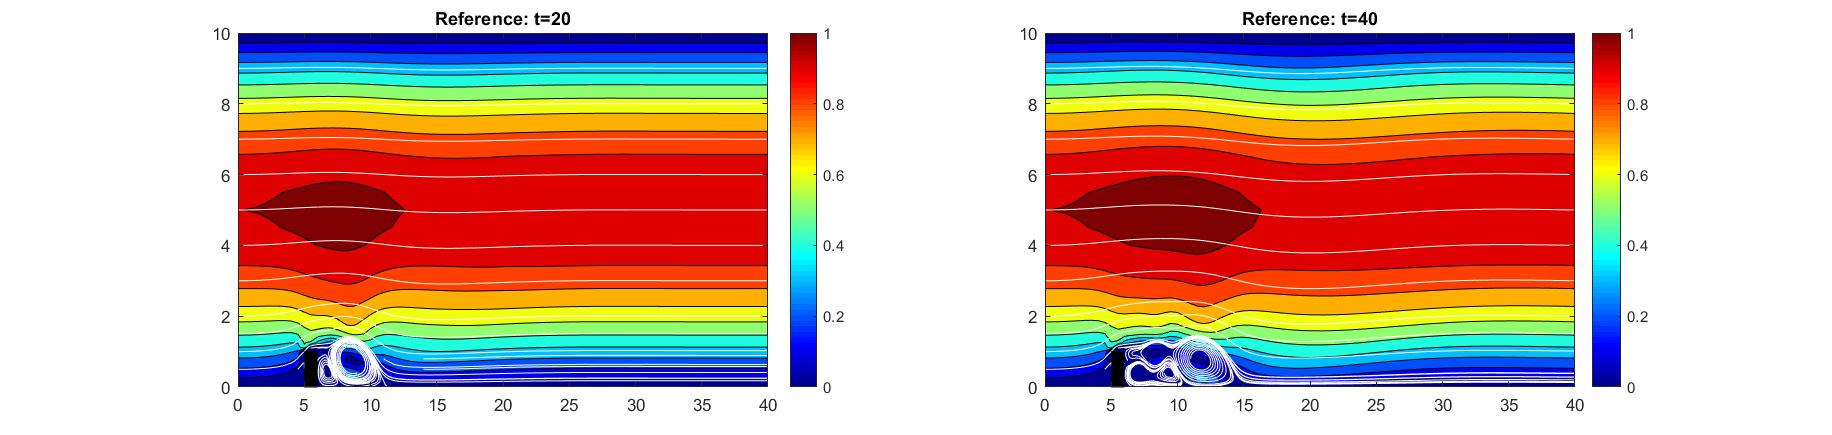
\includegraphics[scale=.13]{step_Skew_fine.jpg}
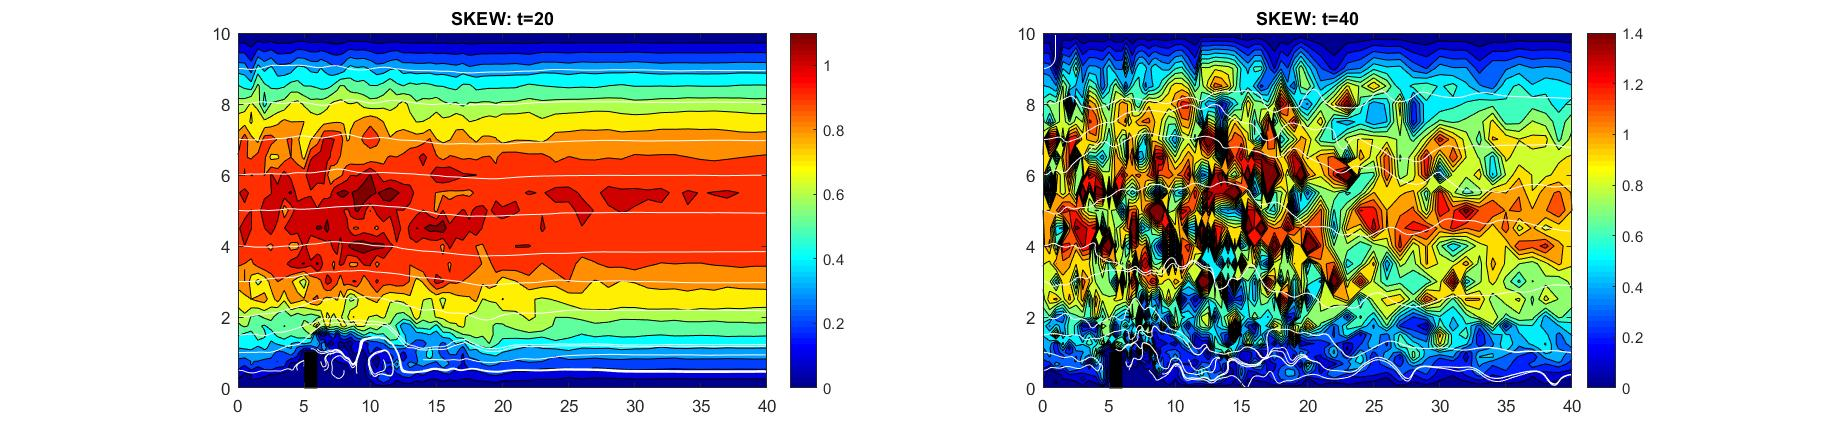
\includegraphics[scale=.13]{step_skew_coarse.jpg}
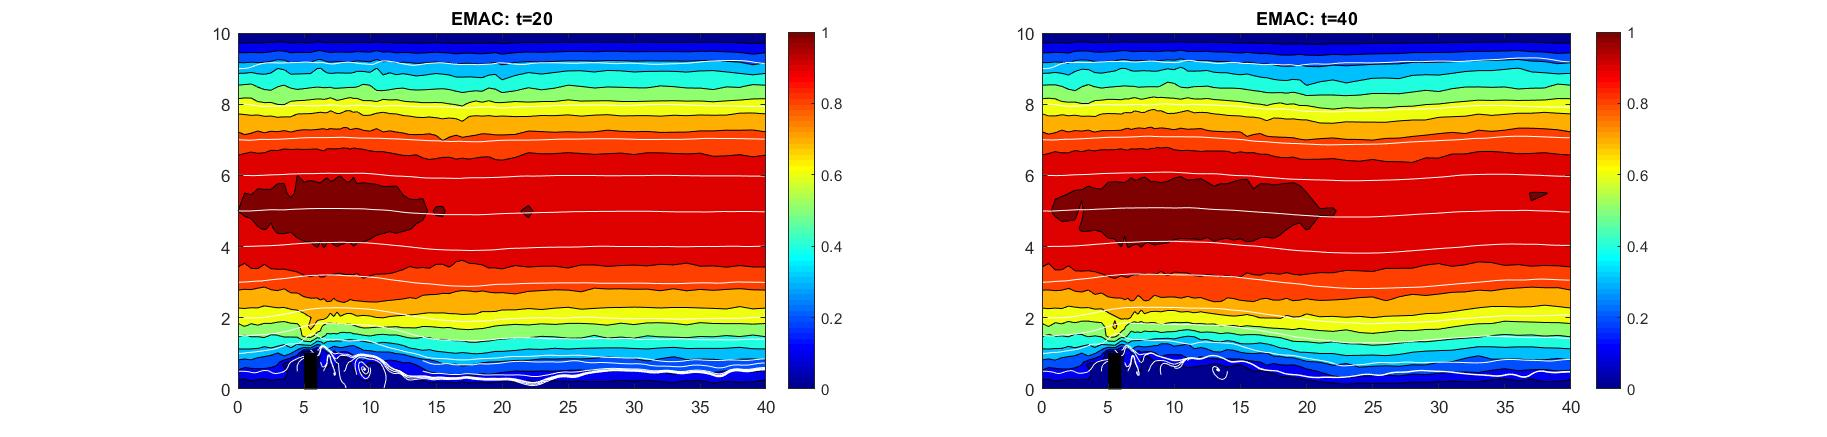
\includegraphics[scale=.13]{step_EMAC_coarse.jpg}
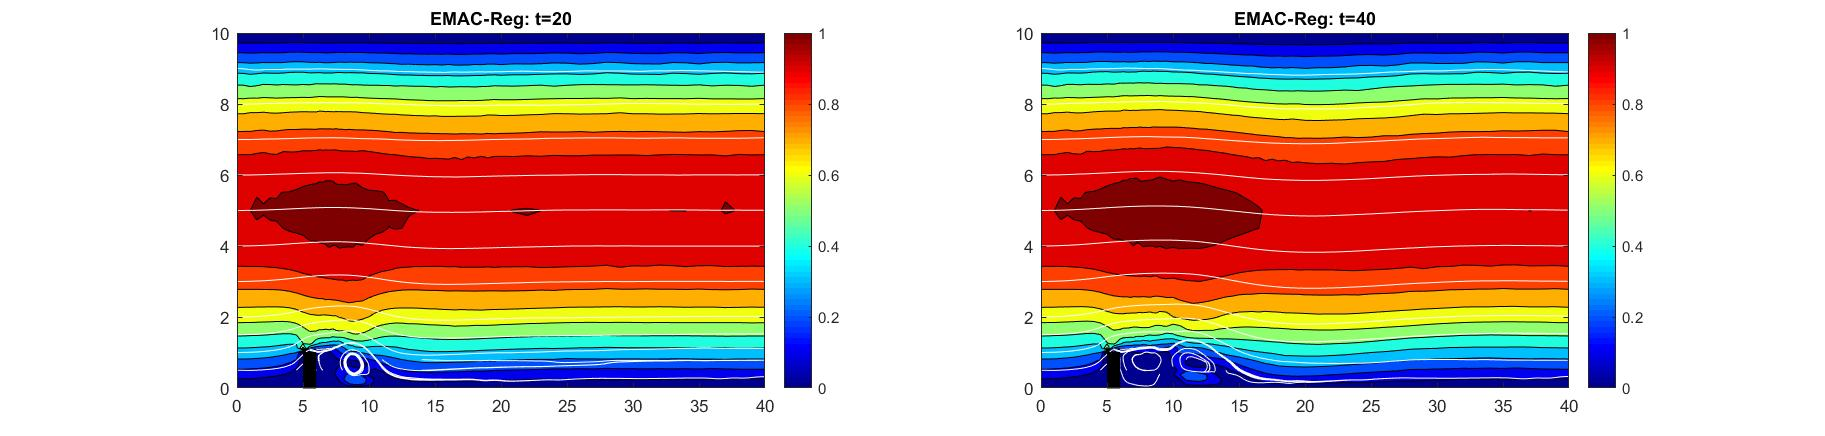
\includegraphics[scale=.13]{step_EMAC_Reg_coarse.jpg}
\end{figure}

\end{frame}

%----------------------------------

\begin{frame}
\frametitle{Results to expect (convergence analysis)}
\begin{align*}
w &= \bmat{-\cos(\pi x)\sin(\pi y)\\ \sin(\pi x)\cos(\pi y)}e^{-2\pi^2\nu t},\\
u &= (1+2\pi^2\alpha^2)w,\\
p &= -w \cdot \nabla w,
\end{align*}
\begin{table}[H]
\begin{scriptsize}
\begin{tabular}{|c||c|c||c|c||}
\hline
h & $\norm{w-w_h}_{\infty,0}$ & Rate & $\norm{w-w_h}_{\infty,1}$ & Rate\\
\hline
1/2 & 3.68383e-02 & - & 6.40968e-01 & -\\
\hline
1/4 & 8.01551e-03 & 2.20034 & 2.15719e-01 & 1.57110\\
\hline
1/8 & 7.40875e-04 & 3.43549 & 4.88487e-02 & 2.14276\\
\hline
1/16 & 8.07978e-05 & 3.19684 & 1.13421e-02 & 2.10663\\
\hline
1/32 & 9.78736e-06 & 3.04532 & 2.77000e-03 & 2.03374\\
\hline
1/64 & 1.21936e-06 & 3.00480 & 6.89712e-04 & 2.00582\\
\hline
1/128 & 1.64691e-07 & 2.88829 & 1.72432e-04 & 1.99996\\
\hline
\end{tabular}
\end{scriptsize}
\caption{Convergence results for both $u$ and $w$ for EMAC-Reg (should be similar to EMAC)}
\label{fig:convergence}
\end{table}
\end{frame}

%----------------------------------

\begin{frame}
\frametitle{Results to expect (Computed Quantities)}
\begin{figure}
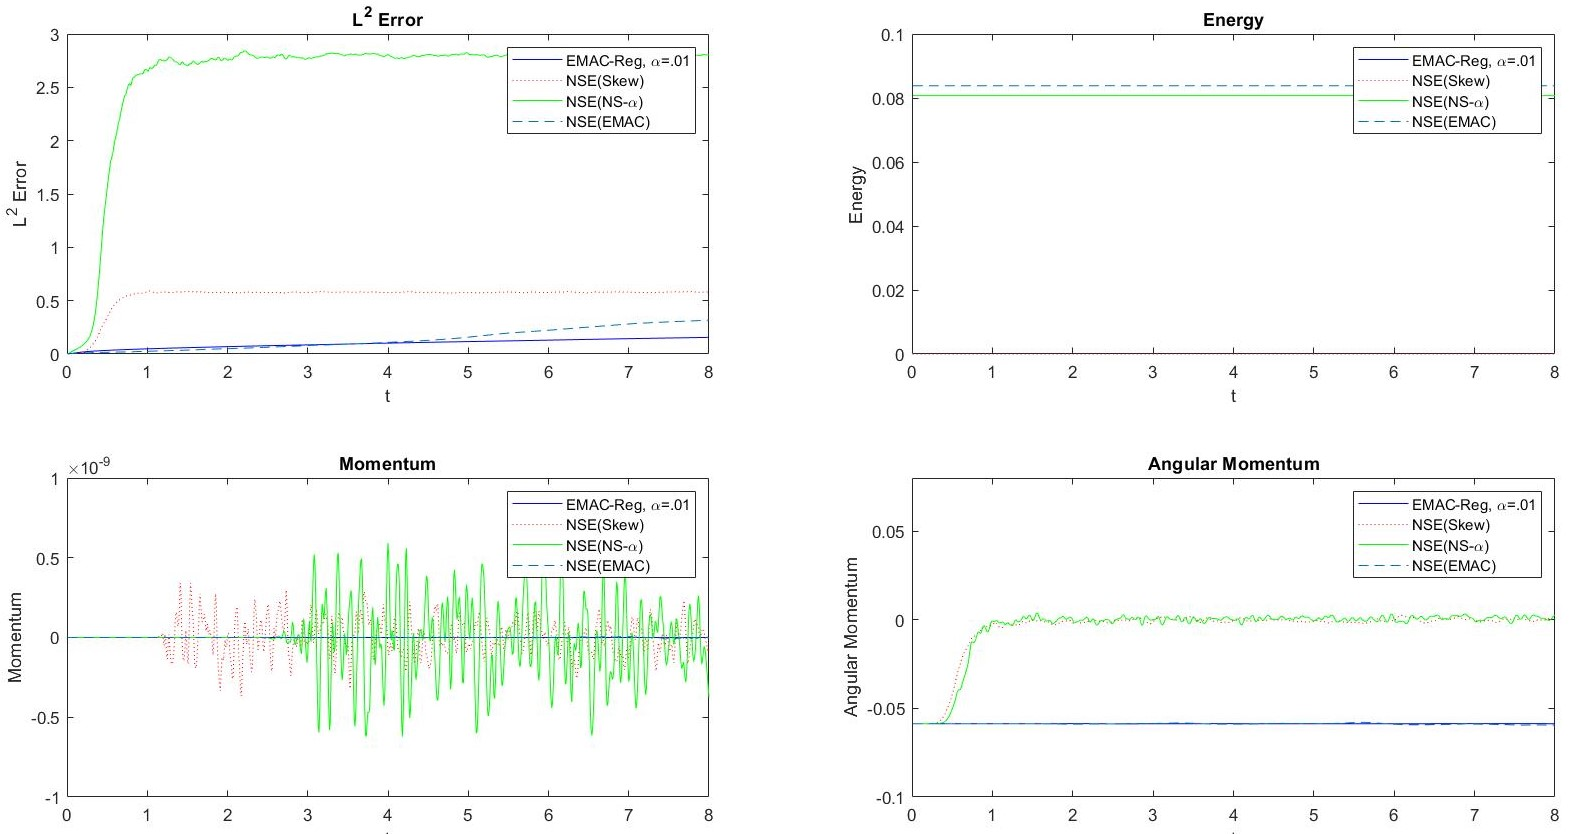
\includegraphics[scale=.25]{Quant_Comparison.jpg}
\end{figure}
\end{frame}

%----------------------------------

\begin{frame}
\frametitle{General idea of step 57}
\begin{itemize}
\item Nonlinear term ($u \cdot \nabla u$) in NSE is problematic
\item Spatially discretize so we get
\begin{align*}
u \cdot \nabla u \approx u_k \cdot \nabla u_{k+1} + u_{k+1} \cdot \nabla u_k - u_k \cdot \nabla u_k
\end{align*}
\item Convergence is quadratic, expect convergence in 2-3 iterations
\item Do the same exact thing for EMAC formulation
\begin{align*}
2D(u)u &\approx 2D(u_k)u_{k+1} + 2D(u_{k+1})u_k - 2D(u_k)u_k\\
(\divergence u)u &\approx (\divergence u_k)u_{k+1} + (\divergence u_{k+1})u_k - (\divergence u_k)u_k
\end{align*}

\end{itemize}
\end{frame}

%----------------------------------

\begin{frame}
\frametitle{Time implementation}
\begin{figure}
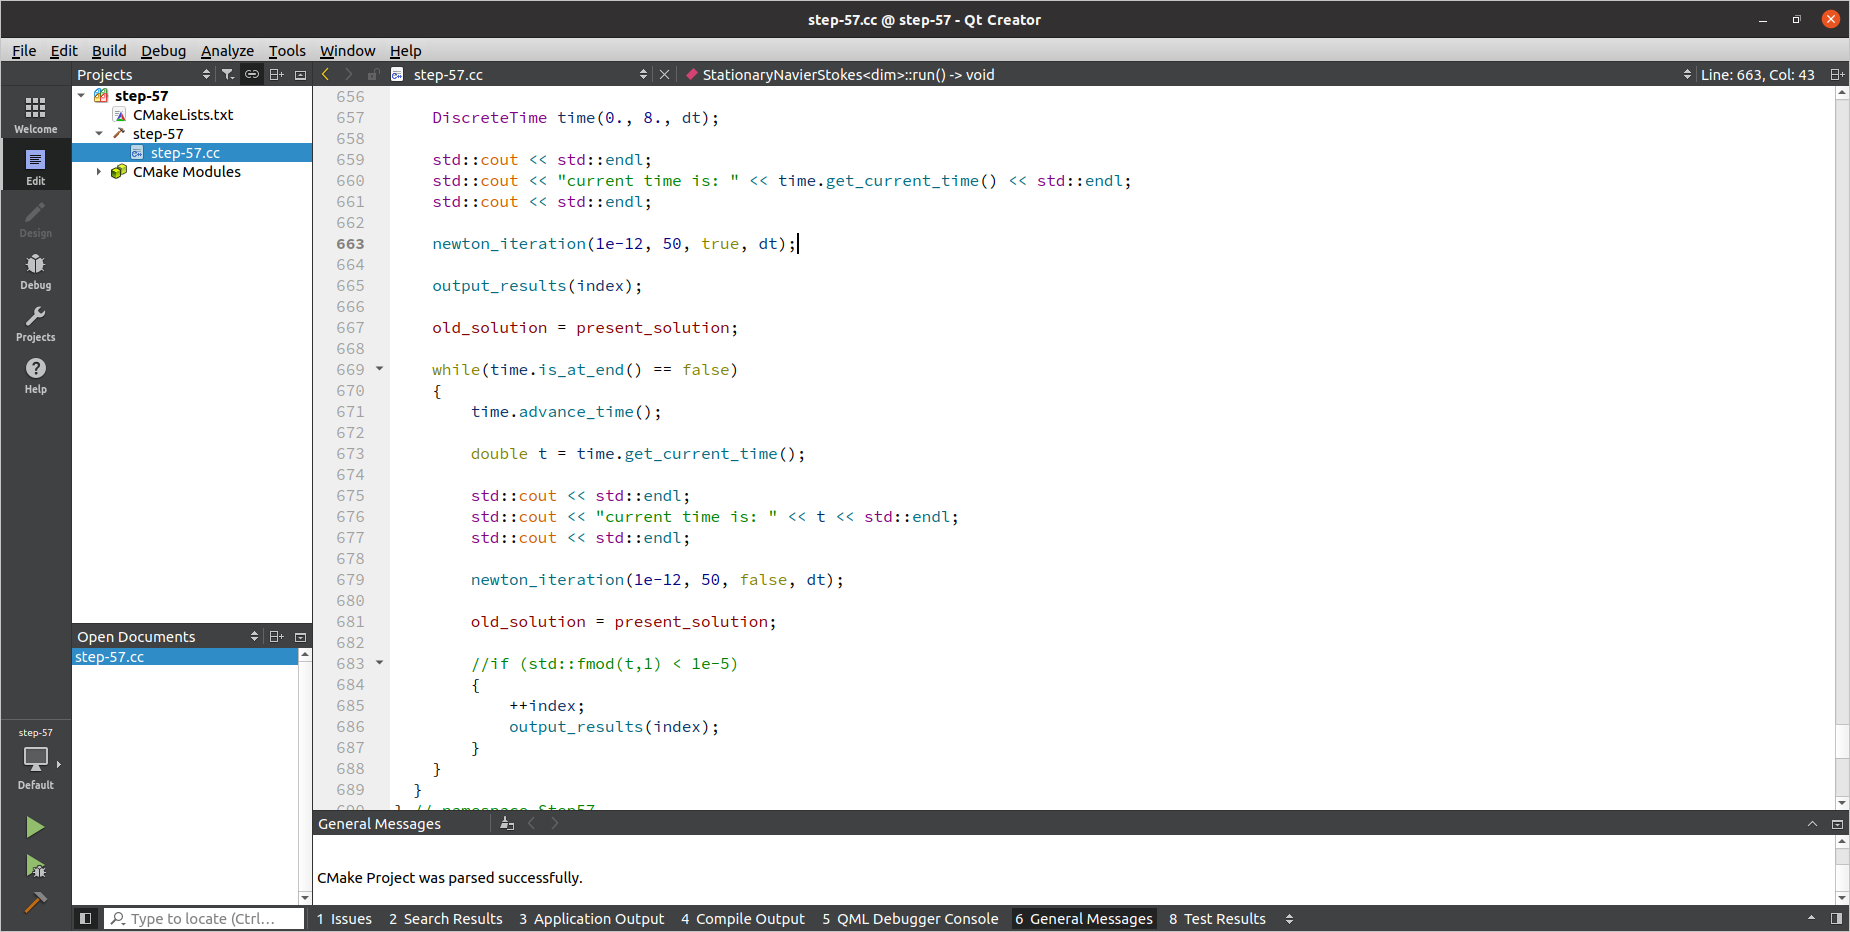
\includegraphics[scale=.18]{time_code.png}
\end{figure}
\end{frame}

%----------------------------------

\begin{frame}
\frametitle{NSE assembly (Identical to step-57)}
\begin{figure}
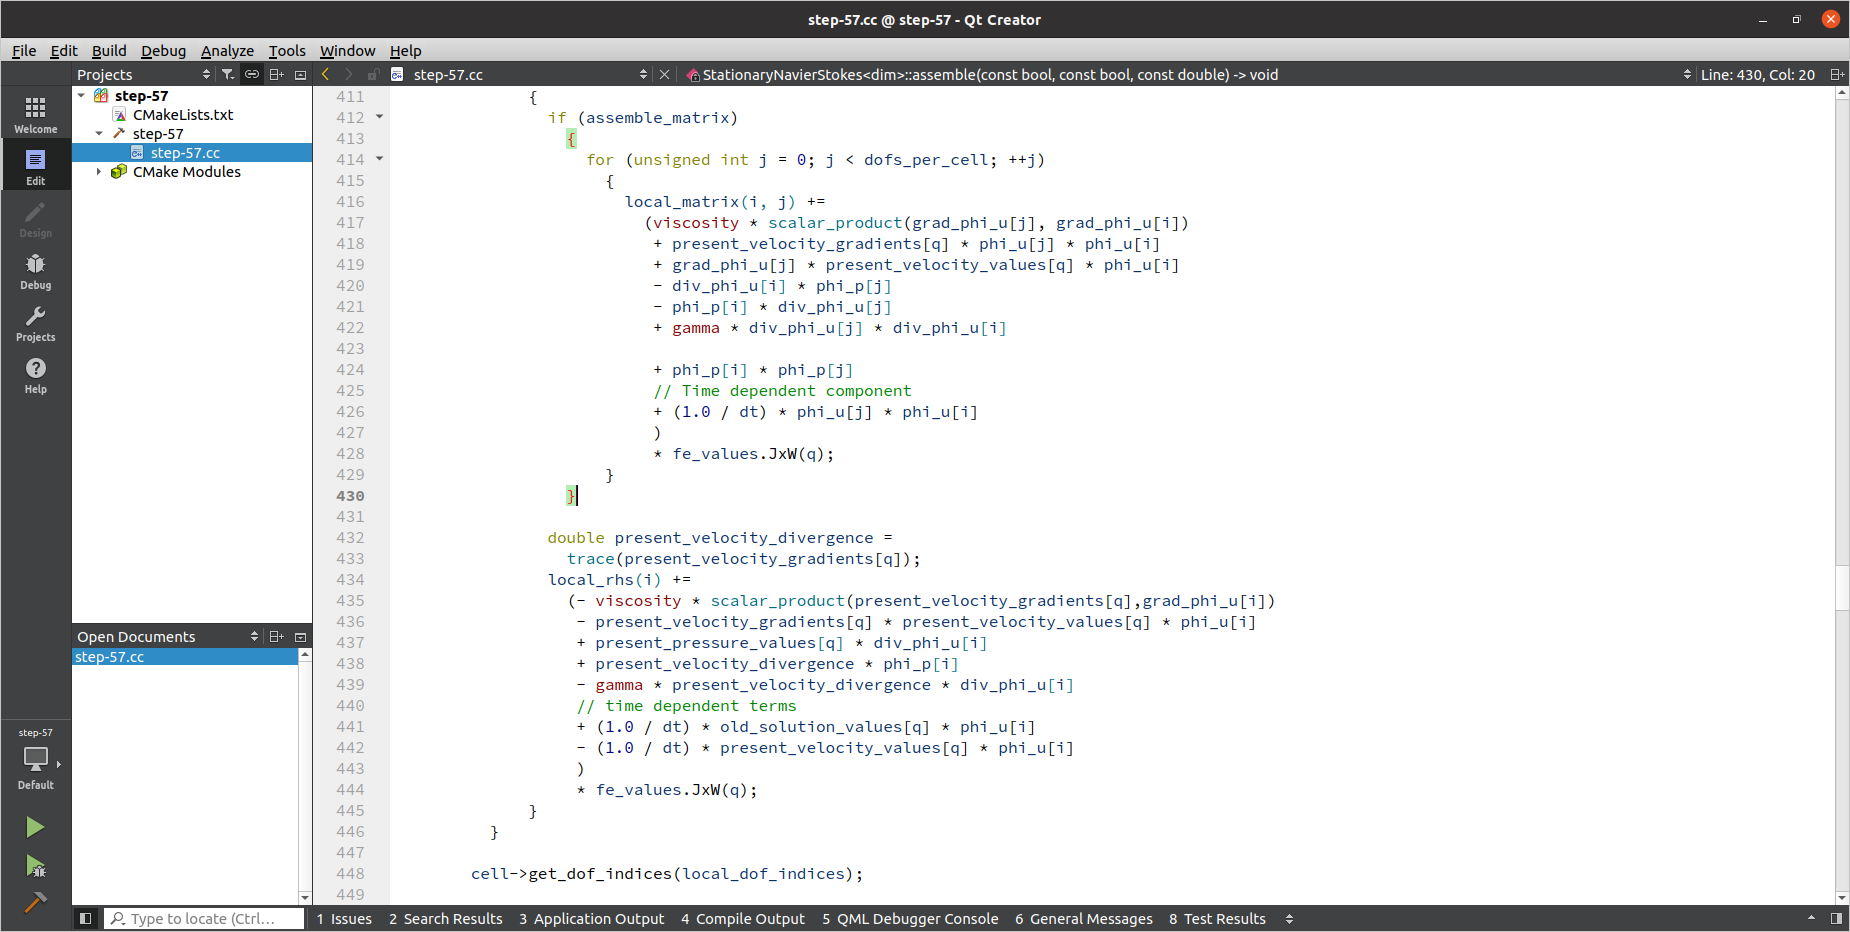
\includegraphics[scale=.18]{NSE_code.png}
\end{figure}
\end{frame}

%----------------------------------

\begin{frame}
\frametitle{EMAC assembly}
\begin{figure}
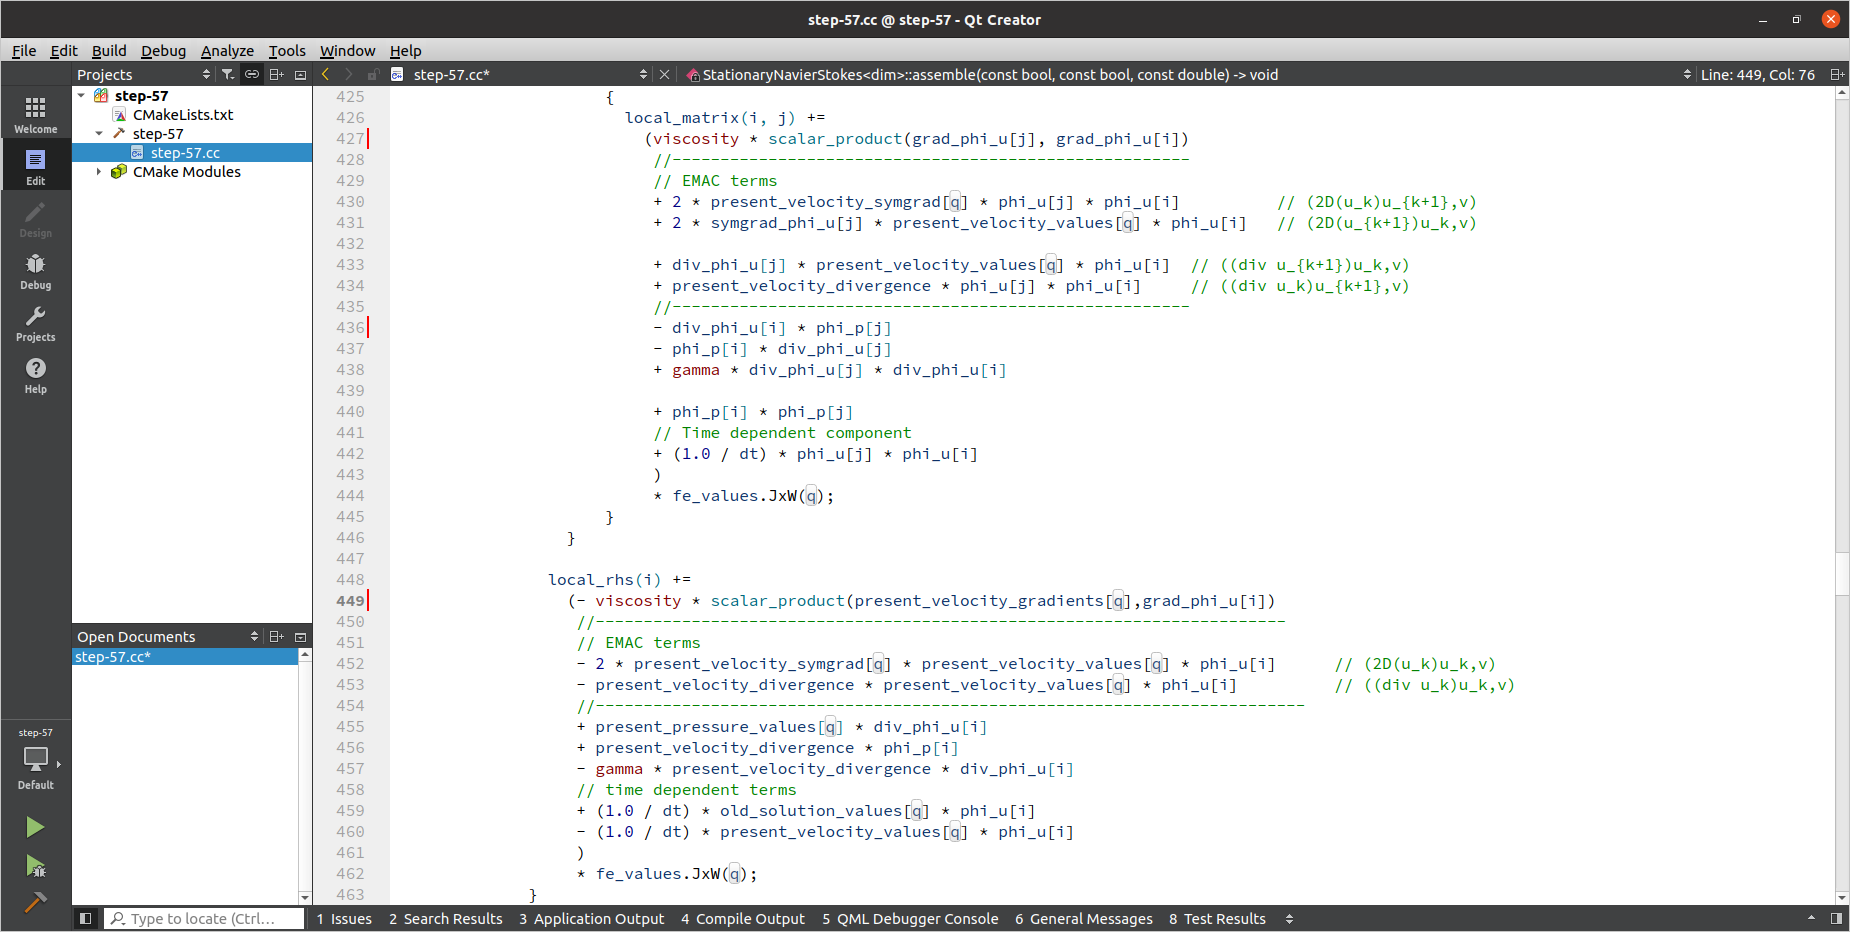
\includegraphics[scale=.18]{EMAC_code.png}
\end{figure}
\end{frame}

%----------------------------------

\begin{frame}
\frametitle{Future work}
\begin{itemize}
\item Implement EMAC-Reg, test in 3D to see coarse mesh effectiveness.
\item Implement MPI, solving on one core in 3D is incredibly inefficient.
\item Calculate energy, momentum, and angular momentum for appropriate problem in deal.II.
\item Implement benchmark problem from slide 6.
\end{itemize}
\end{frame}

%----------------------------------

\end{document}
